\chapter{WAMIT: Output Files}
\label{chap:WamitOutput}


\begin{table}[H]
   \centering
   \caption[Notation for WAMIT output files]{Notation for data contained in the WAMIT output files.  Here $\bar{F}$ is the force quadratic transfer function. The units listed are those given within the WAMIT manual\cite{WAMIT}. Note: some variable names appear differently here than in the WAMIT manual.\label{tab:WamitOutputUnits}}
   \begin{tabular}{cll}
      \toprule
         Variable                   &  Type                       &  Units             \\
      \midrule
         $\tau$                     &  Wave period                &  Seconds           \\
         $\beta$                    &  Wave direction             &  Degrees           \\
         $k$                        &  Force component            &  None              \\
         $\left|\bar{F}\right|$     &  Force QTF Magnitude        &  Nondimensional    \\
         $\theta$                   &  Force QTF Phase            &  Degrees           \\
         $\Re(\bar{F})$             &  Force QTF Real part        &  Nondimensional    \\
         $\Im (\bar{F})$            &  Force QTF Imaginary part   &  Nondimensional    \\     
%         $\rho$                     &  Density of fluid           &  kg/m$^3$          \\
%         $g$                        &  Gravitational constant     &  m/s$^2$           \\
%         $L$                        &  Characteristic length      &  m                 \\
      \bottomrule
   \end{tabular}
\end{table}





WAMIT can use several methods to calculate the normalized second order wave force.  Each of those methods produces a different type of output file.  The calculation methods available to the WAMIT2 module are limited by the WAMIT output files that are available.  \Cref{tab:Wamit2MethodsByFileType} shows what second order force calculation methods are available depending on the WAMIT files available\cite{WAMIT}.
\Cref{tab:WamitOutputUnits} lists the variables used in this document to refer to the various WAMIT outputs.  Note that the notation here differs with the notation used in the WAMIT manual and in Tiago's writings\cite{duarte:2014,WAMIT}.

\section{WAMIT Output}
\Cref{tab:WamitOutputFormat} lists the format for each of the WAMIT output files.
Within these files, the angles and frequencies do not need to be evenly spaced.  Also, it should also be noted that the discretization between $\omega_1$ and $\omega_2$ are not necessarily the same.  This also applies to the angles $\beta_1$ and $\beta_2$.

A value for the period $\tau = 0$ in the WAMIT output file means that the frequency $\omega = \infty$.  A period of $\tau < 0$ is used in the WAMIT output file to indicate $\omega = 0$.

The QTF in the WAMIT output files does not need to be complete since the following relationships are true:
\begin{equation}
   \bar{F}^\text{-}_{mn} = \bar{F}^{\text{-}~*}_{nm}   \qquad \text{and} \qquad   \bar{F}^{+}_{mn} = \bar{F}^{+}_{nm},
\label{eq:WAMIT:QTF_sym}
\end{equation}
where $*$ indicates the complex conjugate.  Note that this implies that the diagonal terms in the second order difference QTF, $\bar{F}^\text{-} (\omega_m,\omega_m) =\bar{F}^{\text{-}~*} (\omega_m,\omega_m)$, are real valued.

The normalized second order wave force in the WAMIT output files is non-dimensional (see Ref~\cite{WAMIT} section 11.6 for details).  These are written as
\begin{equation}
   \bar{F}_k^\text{-}   = \frac{\tilde{F}_k^\text{-}}{\rho g L^a A_m A^*_n} 
         \qquad\text{and}\qquad
   \bar{F}_k^{+}        = \frac{\tilde{F}_k^{+}}{\rho g L^a A_m A_n},
\label{eq:QTF:nondimensional}
\end{equation}
where $a=1$ for forces ($k = 1, 2, 3$) and $a=2$ for moments ($k=4, 5, 6$), $\bar{F}_k$ and $\tilde{F}_k$ are respectively the non-dimensioned and dimensioned QTFs for the $k^\text{th}$ force component, 
and $A_m$ and $A^*_n$ are the complex wave and complex conjugates of the amplitudes. Other variables are listed in \Cref{tab:2ndOrdNotation}.
In order to simplify using the dimensioned wave force in calculations, \Cref{eq:QTF:nondimensional} can be rewritten as
\begin{equation}
    \tilde{F}_k^\text{-}   = A_m A^*_n \left(\bar{F}_k^\text{-}   \rho g L^a\right)    = A_m A^*_n  {F}_k^\text{-} 
         \qquad\text{and}\qquad
     \tilde{F}_k^+         = A_m A_n   \left(\bar{F}_k^+          \rho g L^a\right)    = A_m A_n    {F}_k^+,
\label{eq:QTF:dimensional}
\end{equation}
where ${F}_k^\pm$ is partially dimensioned by $\rho g L^a$, but does not include the wave amplitudes.


\newcommand{\pboxl}[1]{\footnotesize{\parbox[c]{1.35in}{#1}}}
\begin{table}
   \centering
   \caption[Format of WAMIT output files]{WAMIT output files and format (version 6.4/6.1s)\cite{WAMIT}. In this table, $\tau$ is the period of the wave, $\beta_m$ and $\beta_n$ are the wave directions.  The second order complex force term is given by both the amplitude and phase pair ($\left|\bar{F}_m\right|$ and  $\theta_m$), and in terms of its real and imaginary parts ($\Re (\bar{F}_m)$ and $\Im (\bar{F}_m)$).  The index $k$ indicates the force ($k=1\ldots3$) or moment ($k=4\ldots6$) load components.  The indices $m$ and $n$ correspond to the period of the waves that are interacting (see pages 4-9 and 11-13 of Ref.~\citen{WAMIT}).\label{tab:WamitOutputFormat}}
   \tabcolsep=1.75mm
   \begin{tabular}{c>{\raggedright}p{1.35in}ccccccccc}
      \toprule
 File Ext.  &  Description    &  \multicolumn{9}{l}{Output Format} \\
%         File  &                 & \multicolumn{2}{c}{Period}  & \multicolumn{2}{c}{Angle}            & DOF & Ampl.  & Phase  & Real   & Imag.  \\
%         Ext.  &  Description    & \multicolumn{2}{c}{(s)} & \multicolumn{2}{c}{(deg)} & (-) & (-)    & (rad?) & (-)    & (-)    \\
      \midrule
   .7       &  {\pboxl{Mean drift based on momentum flux (WAMIT v. 7 only)}}
            &  $\tau_m$ &                          &  $\beta_{m(1)}$    &  $\beta_{m(2)}$                &  $k$   
            &  $\left|\bar{F}^{-}_{mm}\right|$     &  $\theta_{mm}$     &  $\Re (\bar{F}^{-}_{mm})$      &  $\Im (\bar{F}^{-}_{mm})$      \\[7pt]
   .8       &  {\pboxl{Mean drift (modes 1, 2, and 6)}}
            &  $\tau_m$ &                          &  $\beta_{m(1)}$    &  $\beta_{m(2)}$                &  $k$   
            &  $\left|\bar{F}^{-}_{mm}\right|$     &  $\theta_{mm}$     &  $\Re (\bar{F}^{-}_{mm})$      &  $\Im (\bar{F}^{-}_{mm})$      \\[5pt]
   .9       &  {\pboxl{Mean drift (all modes)}}
            &  $\tau_m$ &                          &  $\beta_{m(1)}$    &  $\beta_{m(2)}$                &  $k$   
            &  $\left|\bar{F}^{-}_{mm}\right|$     &  $\theta_{mm}$     &  $\Re (\bar{F}^{-}_{mm})$      &  $\Im (\bar{F}^{-}_{mm})$      \\[1pt] \midrule
   .10s     &  {\pboxl{Quadratic \nth{2}-order sum forces}}
            &  $\tau_m$ &  $\tau_n$                &  $\beta_{m}$       &  $\beta_n$                     &  $k$   
            &  $\left|\bar{F}_{mn}^{+}\right|$     &  $\theta_{mn}^{+}$ &  $\Re (\bar{F}_{mn}^{+})$      &  $\Im (\bar{F}_{mn}^{+})$      \\[5pt]
   .10d     &  {\pboxl{Quadratic \nth{2}-order difference forces}}
            &  $\tau_m$ &  $\tau_n$                &  $\beta_{m}$       &  $\beta_n$                     &  $k$   
            &  $\left|\bar{F}_{mn}^{-}\right|$     &  $\theta_{mn}^{-}$ &  $\Re (\bar{F}_{mn}^{-})$      &  $\Im (\bar{F}_{mn}^{-})$      \\[5pt]
   .11s     &  {\pboxl{Total \nth{2}-order forces by indirect method (sum)}}
            &  $\tau_m$ &  $\tau_n$                &  $\beta_{m}$       &  $\beta_n$                     &  $k$   
            &  $\left|\bar{F}_{mn}^{+}\right|$     &  $\theta_{mn}^{+}$ &  $\Re (\bar{F}_{mn}^{+})$      &  $\Im (\bar{F}_{mn}^{+})$      \\[7pt]
   .11d     &  {\pboxl{Total \nth{2}-order forces by indirect method (diff)}}
            &  $\tau_m$ &  $\tau_n$                &  $\beta_{m}$       &  $\beta_n$                     &  $k$   
            &  $\left|\bar{F}_{mn}^{-}\right|$     &  $\theta_{mn}^{-}$ &  $\Re (\bar{F}_{mn}^{-})$      &  $\Im (\bar{F}_{mn}^{-})$      \\[7pt]
   .12s     &  {\pboxl{Total \nth{2}-order forces by direct method (sum)}}
            &  $\tau_m$ &  $\tau_n$                &  $\beta_{m}$       &  $\beta_n$                     &  $k$   
            &  $\left|\bar{F}_{mn}^{+}\right|$     &  $\theta_{mn}^{+}$ &  $\Re (\bar{F}_{mn}^{+})$      &  $\Im (\bar{F}_{mn}^{+})$      \\[7pt]
   .12d     &  {\pboxl{Total \nth{2}-order forces by direct method (diff)}}
            &  $\tau_m$ &  $\tau_n$                &  $\beta_{m}$       &  $\beta_n$                     &  $k$   
            &  $\left|\bar{F}_{mn}^{-}\right|$     &  $\theta_{mn}^{-}$ &  $\Re (\bar{F}_{mn}^{-})$      &  $\Im (\bar{F}_{mn}^{-})$      \\
      \bottomrule
   \end{tabular}
\end{table}






\section{Reading WAMIT Data Files}
\label{sec:WamitOuput:Read}
\todo[inline]{Make pretty version of \Cref{fig:2ndOrdRead}}

\subsection{First order WAMIT output files (.3)}
The algorithm used in reading in the first order WAMIT data files involves scanning through the data file multiple times.  This is roughly summarized as:
\begin{enumerate}
   \item{Get wave period information}
   \begin{enumerate}
      \item{Read through file to find the number of wave periods}
      \item{Allocate array to hold the wave periods in the order they appear in the file (\varname{WAMITPer} and \varname{WAMITFreq})}
      \item{Allocate array \varname{SortFreqInd} to hold the ordered indices of the sorted frequencies}
      \item{Allocate array \varname{HdroFreq} to hold the sorted frequencies}
      \item{Read through file to populate the \varname{WAMITPer}, \varname{WAMITFreq} and \varname{SortFreqInd} arrays}
      \item{Read through file and store the sorted frequencies in \varname{HdroFreq}}
   \end{enumerate}
   \item{Get wave directions}
   \begin{enumerate}
      \item{Read through first wave period to get the directions}
      \item{Allocate array to hold the wave directions in the order they appear in the file (\varname{WAMITDir})}
      \item{Allocate array \varname{SortWvDirInd} to hold the ordered indices of the sorted directions}
      \item{Allocate array to hold the ordered indices of the sorted directions (\varname{HdroWvDir})}
      \item{Read through file to populate \varname{WAMITDir} and assemble}
      \item{Read through file and store the sorted directions in \varname{HdroWvDir}}
   \end{enumerate}
   \item{Populate the complex wave information \varname{HdroExctn}}
   \begin{enumerate}
      \item{Read through the file again to populate \varname{HdroExctn}(\varname{SortFreqInd}(K),\varname{SortWvDirInd}(J),I)}
   \end{enumerate}
\end{enumerate}

There are two subtle assumptions about the organization of the WAMIT output file that are made here.  First, the file is always organized such that the wave direction is looped through for each value of the wave period.  The second assumption is that all the force components are grouped for a given wave direction and wave period.  In the case of the second order WAMIT data, this may not be true.

\subsection{Second order WAMIT output files}

The calculations for the second order WAMIT output are very time consuming.  In order to help alleviate this problem, WAMIT allows the user to specify exactly which combinations of wave heading and wave periods to calculate in a .PT2 input file.  As a result, the output file may be very sparse, and may not be ordered in any meaningful way.  Therefore, a different approach that does not make assumptions about the ordering of the file should be used.

\begin{figure}[H]
   \centering
   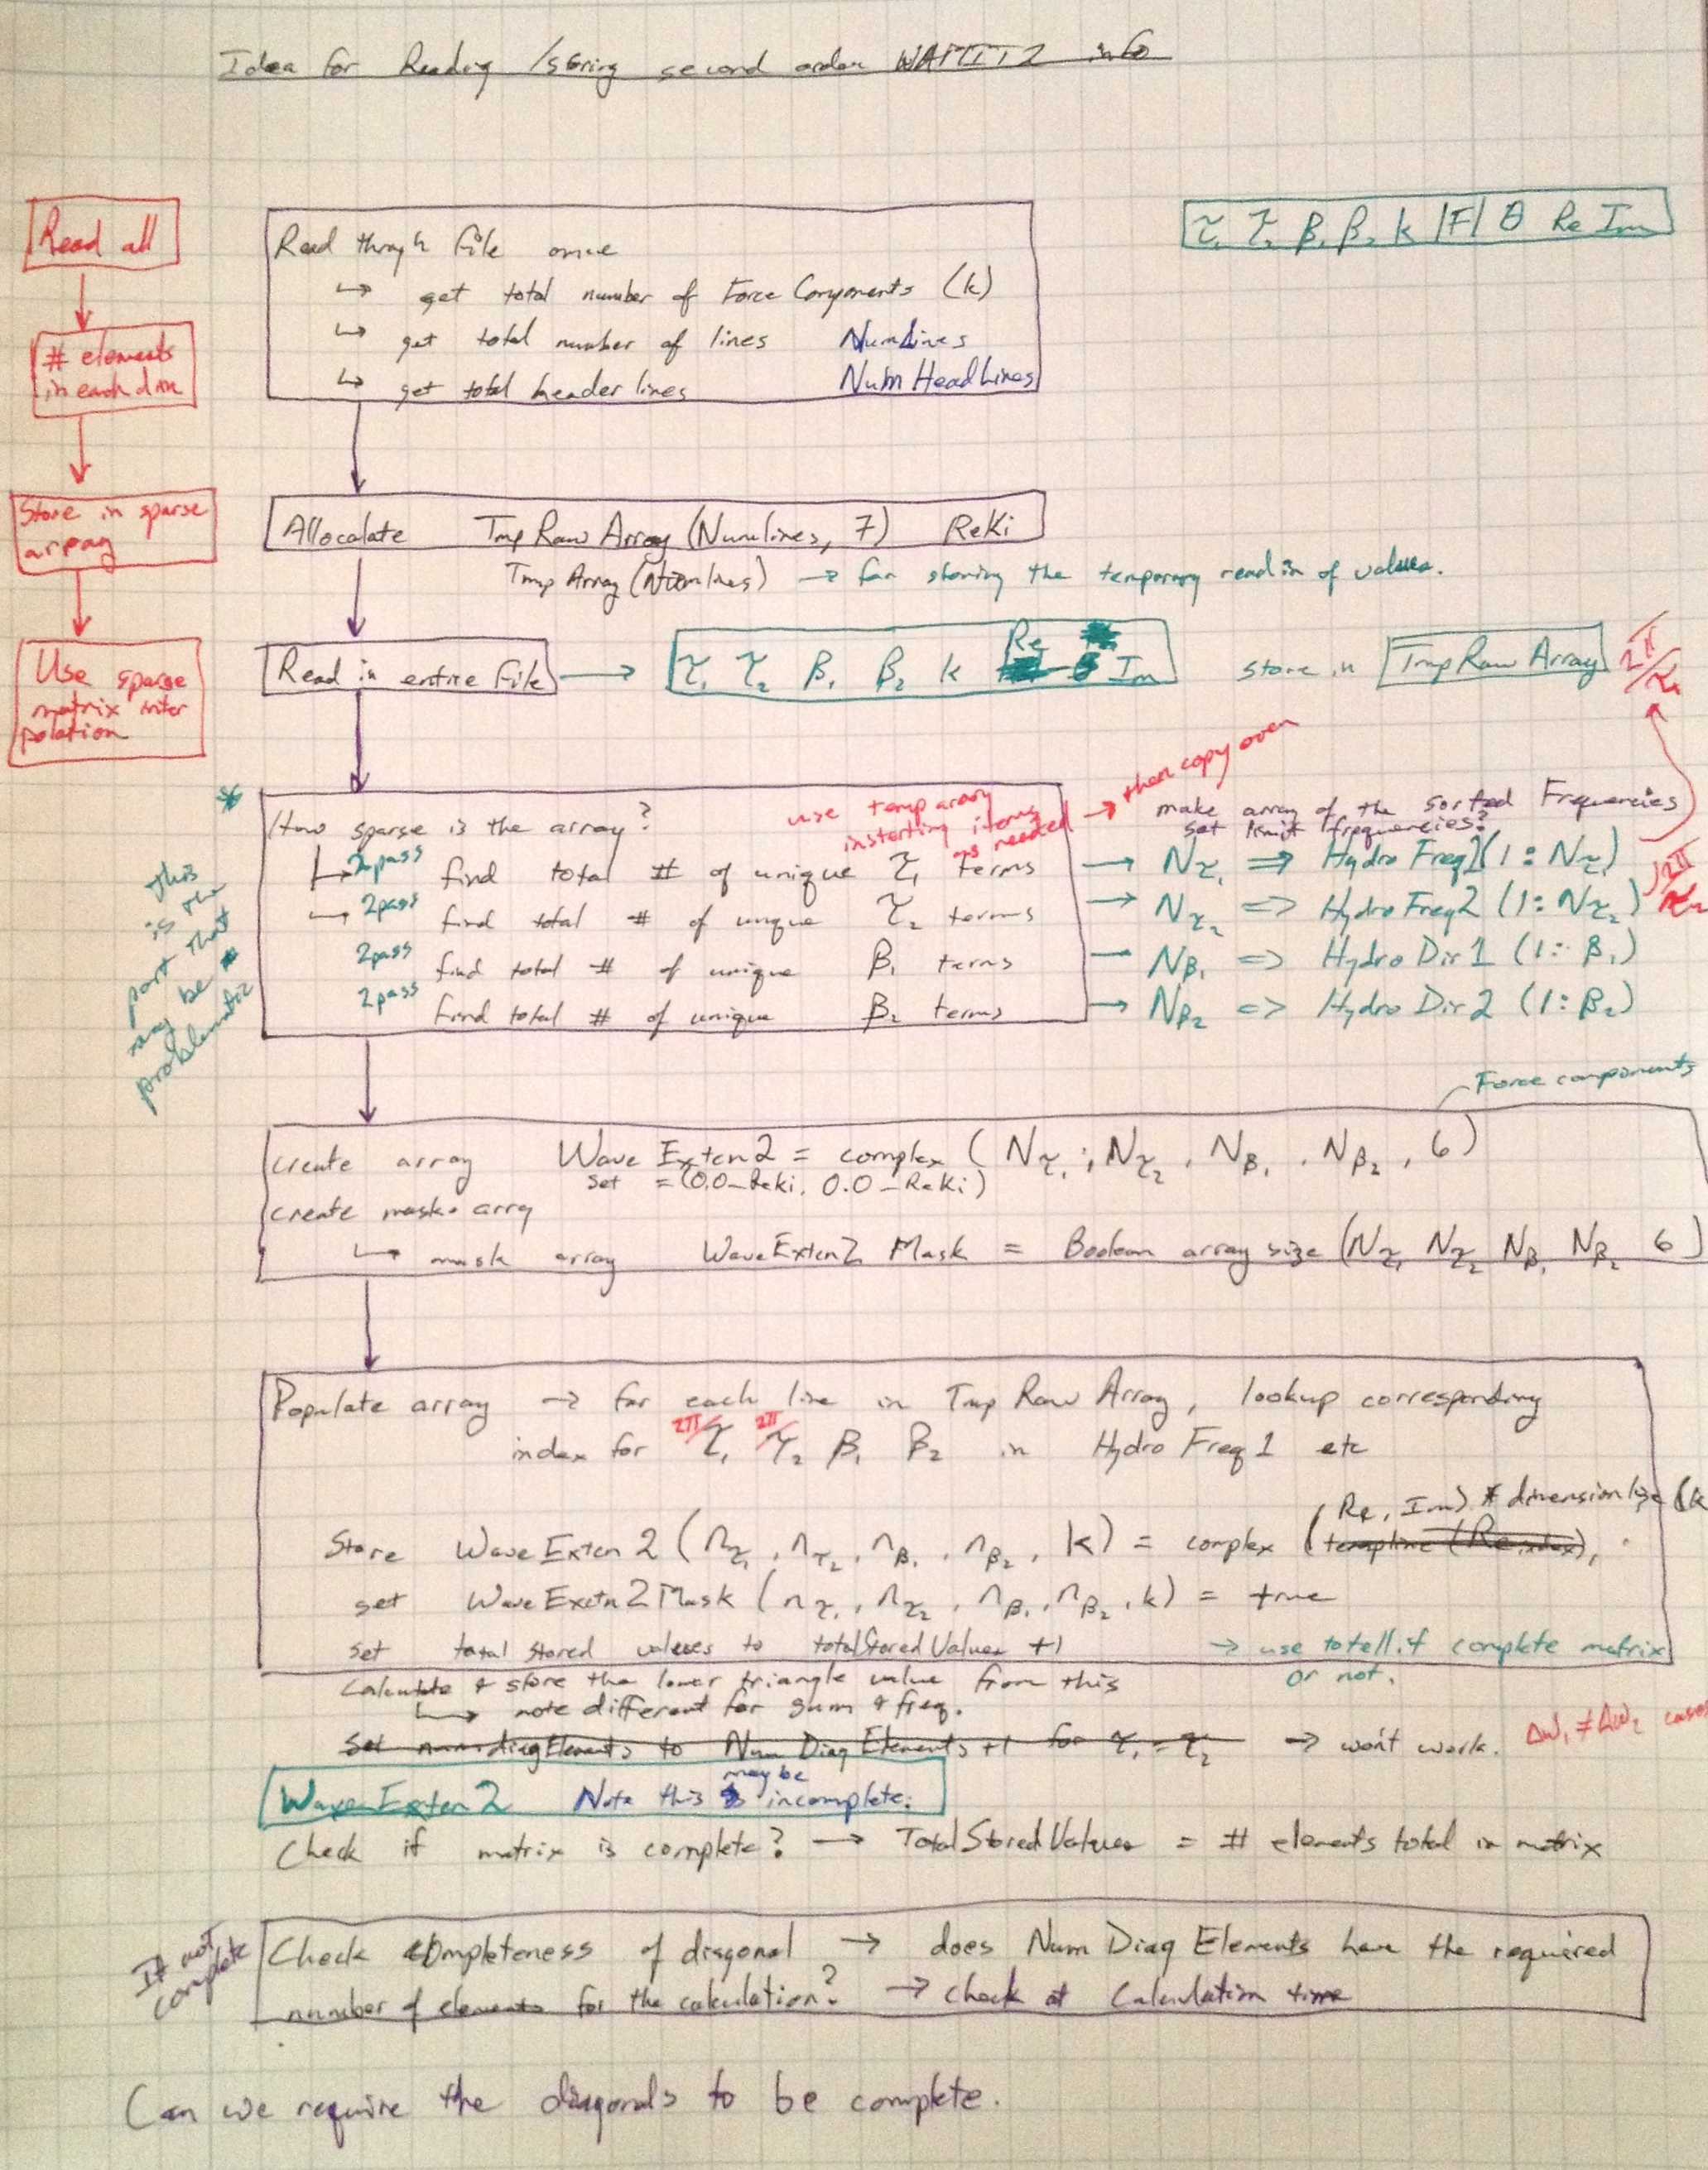
\includegraphics[height=8in]{chaps/figures/WAMIT2--read_Algorithm.jpg}
   \caption{Overview of scheme for reading in 2nd order WAMIT files with two periods (.10, .11, .12).  The algorithm for reading in 2nd order WAMIT files with only one period (.7, .8, .9) should be a simplified version of this algorithm.
      \label{fig:2ndOrdRead}}
\end{figure}

The overall idea of this approach is to read the entire data file a temporary array in memory, and then figure out how many unique values of $\omega_1, \omega_2, \beta_1,$ and $\beta_2$ there are.  Once this has been determined, the arrays storing the sorted frequencies and directions can be allocated along with the array for storing $F^\pm$.  In addition to the array holding the data, a mask array (boolean?) of equal size must be created to store information regarding which values are populated.  This will be necessary for knowing how sparse the array is and for interpolation algorithms that can handle limited sparseness.

Due to the number of times the file would need to be read for this algorithm, it will likely be faster to read everything into memory and then process rather than rewind the file many times (disk IO is slow).  This does impose some memory usage that could be avoided, but given how long it takes WAMIT to perform these calculations, the files are likely to be small (at least in comparison to the wind files).


\clearpage

\section{WAMIT Data Integrity Checks}
\label{sec:WamitOutput:Checks}
A few checks can be enforced to ensure that the calculations within the \modname{WAMIT2} module can be performed using the provided data.  If the limits of frequency or wave direction are set outside what is provided within the WAMIT output data, an error should be issued and the program aborted.  This could be checked during the calculations by checking if either $\omega < \min{(\tilde{\omega})}$ or $\omega > \max{(\tilde{\omega})}$ is true, where $\tilde{\omega}$ is the array of frequencies given in the WAMIT output files.  Alternatively, this could be checked immediately after reading the WAMIT output file by checking against the limits in the \HD input file as follows:
\begin{eqnarray}
   \varname{WvLowCOffD} > \min{(\tilde{\omega}_D)}\\
   \varname{WvHiCOffD}  < \max{(\tilde{\omega}_D)}
\label{eq:WAMIT:DataLimitTest:Diff}
\end{eqnarray}
for difference QTF files, and
\begin{eqnarray}
   \varname{WvLowCOffS} > \min{(\tilde{\omega}_S)}\\
   \varname{WvHiCOffS}  < \max{(\tilde{\omega}_S)}
\label{eq:WAMIT:DataLimitTest:Sum}
\end{eqnarray}
for sum QTF files where $\tilde{\omega}_D$ and $\tilde{\omega}_S$ are the arrays of frequencies found in the difference and sum WAMIT files, respectively.

In addition to checking the frequency range of the WAMIT output files, the wave direction range should also be checked.  The values can be checked agains the \varname{WaveDirMin} and \varname{WaveDirMax} variables (derived from \varname{WaveDir} and \varname{WaveDirRange} in the \HD input file -- see \Cref{chap:MultiDir}).  Care needs to be taken to account for a possible boundary between positive and negative direction headings ($\pi$ and $-\pi$ directions).
%\todo{Expand this to include eqs/pseudocode for checking of WAMIT data files}

%note on the header lines




\endinput
\section{Additional Data Requirements for the WAMIT2 Module}
\label{sec:WamitOutput:Req}

We will add some additional requirements for second order WAMIT files as they become evident (\emph{i.e.} frequency limits).



\begin{table}
\end{table}
